

\section{Sensor de Pressão}
\label{pressao}


\begin{table}[ht!]

	\begin{tabular}{r l|l p{12cm} }
		
		\textcolor{gray}{Especificação} &&& 	{Transmissor de Pressão digital
		ultra-preciso - HPXFL}\\
		\textcolor{gray}{Data} &&& 				{03/04/2014}\\
        \textcolor{gray}{Beneficiado} &&&		{Velki} \\
        \textcolor{gray}{CNPJ} &&& 				{08.054.040/0001-28} \\
        \textcolor{gray}{Número Nota} &&& 		{2556,00} \\
		\textcolor{gray}{Quantidade} &&& 		{1} \\
		\textcolor{gray}{Valor} &&& 			{R\$1.6525,50} \\
		\textcolor{gray}{Data Sheet} &&& 		{Anexo V - \ref{datasheet_pressao} } \\

		\textcolor{gray}{Função no projeto} &&& {O sensor de pressão será utilizado
		para medir a profundidade do robô durante o processo de inserção e remoção da
		viga pescadora.} \\
		\textcolor{gray}{Razão da Escolha} &&& {O sensor de pressão da Velki já foi
		utilizado previamente em outros projetos do laboratório. O conhecimento da sua
		eletrônica e protocolo pelo grupo levaram a sua escolha.}
		

	\end{tabular}
\end{table}

\newpage

\begin{figure}[h!]
 \centering
 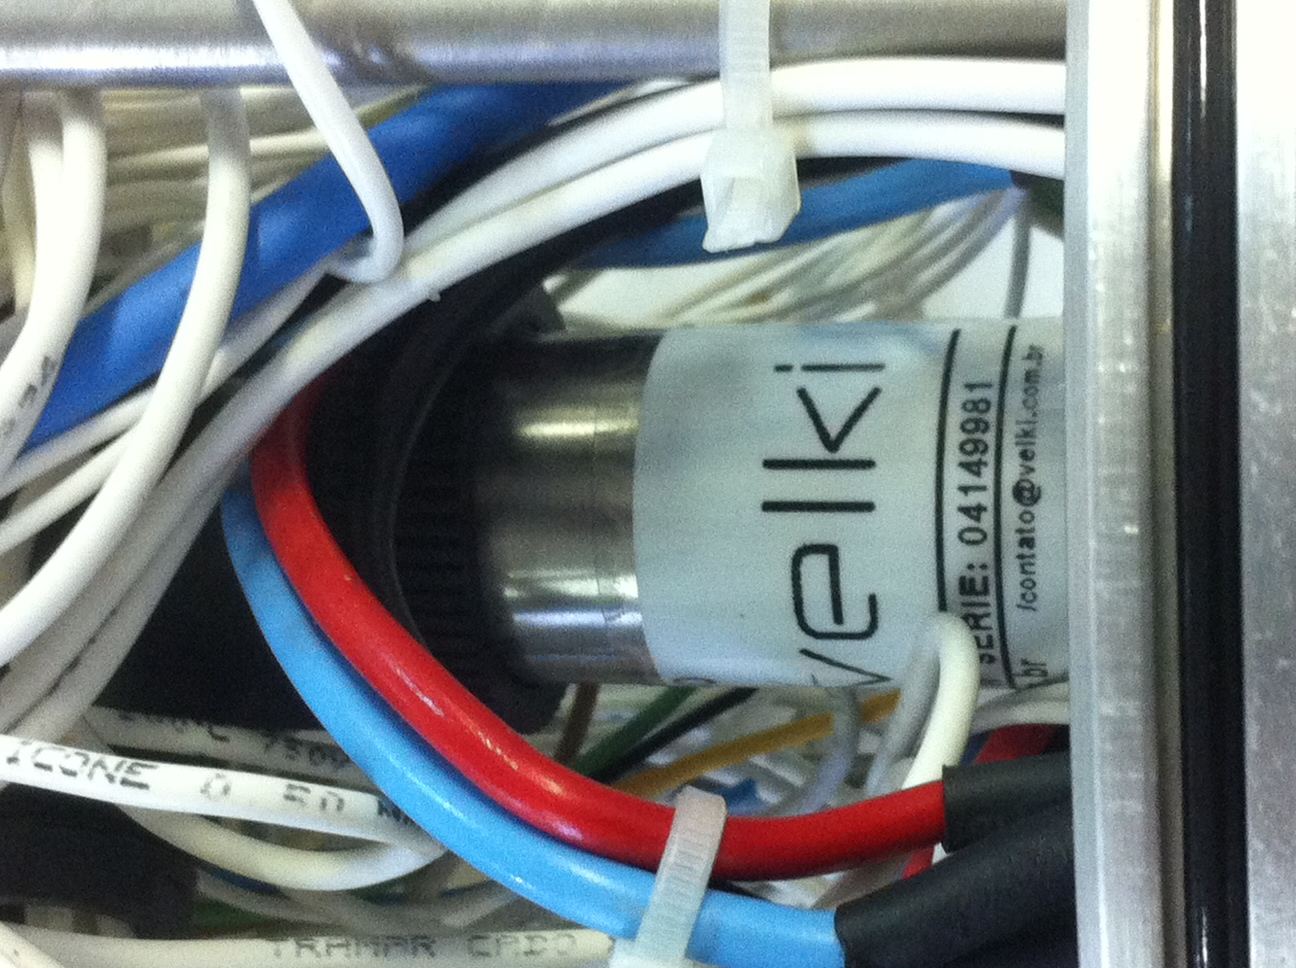
\includegraphics[width=1\columnwidth]{Pressao/foto}
 \caption{Sensor Pressão}
\end{figure}